\documentclass[a4paper,12pt,titlepage]{article}
\usepackage[utf8]{inputenc}
\usepackage{graphicx} % Required for inserting images
\usepackage[spanish,es-tabla]{babel}
\usepackage[none]{hyphenat}
\usepackage[justification=centering]{caption}
\usepackage{subcaption}
\usepackage{amssymb, amsmath}
\usepackage{gensymb}
\usepackage{fancyhdr}

\lhead{Densidad y viscosidad}
\rhead{Gonzalo Bastos González}

\pagestyle{fancy}

\title{Densidad y viscosidad}
\author{Gonzalo Bastos González}

\begin{document}

\maketitle

\tableofcontents
\newpage


\section{Objetivos}

Los objetivos de esta práctica son familiarizarnos con los conceptos de densidad y viscosidad de un líquido, además de trabajar con elementos como un picnómetro o un viscosímetro. La primera parte de la práctica abordará el concepto de densidad y se tratará de conocer las densidades de dos líquidos y un sólido a partir de un líquido de densidad conocida, el agua.
La segunda parte de la práctica abordará el concepto de viscosidad, que se puede entender como la resistencia de ofrece un líquido a fluir. Para ello se realizará un estudio comparativo de la viscosidad de los tres líquidos con los que trabajamos durante toda la práctica: el agua, la acetona y el alcohol.

\section{Materiales y metodología}

\subsection{Densidad}

\begin{itemize}
    \item Picnómetro
    \item Balanza digital
    \item Materiales a estudiar: Agua, acetona, alcohol y perdigones de plomo
\end{itemize}

La primera parte de la práctica consiste en un estudio de la densidad de varios materiales (Acetona, alcohol y plomo) por el método de picnometría. Para ello contaremos con un picnómetro a nuestra disposición de un volumen \textit{a priori} desconocido y que tendremos de calcular. 

\begin{figure}[h!]
    \centering
    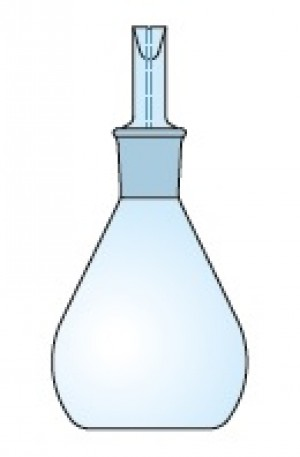
\includegraphics[width=0.30\linewidth]{imágenes/picnometro.jpg}

    \caption{Esquema de un picnómetro}
\end{figure}

Cabe destacar que aunque el volumen del picnómetro venga indicado en el aparato este valor es orientativo y se debe realizar el cálculo del volumen igual ya que, como se podrá observar posteriormente, el valor indicado y el valor real difieren un poco. Para el cálculo del volumen del picnómetro se pesará primero vacío y seco en la balanza y luego se realizarán diez medidas con el picnómetro lleno de agua. En las medidas del picnómetro con agua es importante llenarlo hasta desbordarlo y luego secarlo bien para que el volumen de líquido se mantenga constante siempre y no existan gotas de agua por fuera que interfieran en la medida.

\par Para calcular el volumen vamos a partir del concepto de densidad $(\rho = \frac{m}{V})$ y suponemos que el agua es un líquido de densidad conocida $(\rho_{o} = 1000 \: \frac{kg}{m^3}=1 \: \frac{g}{mL})$, para poder calcular así el volumen de agua que hay en el picnómetro con la siguiente relación:

\begin{equation}
    V = \frac{m-m_{p}}{\rho_{o}}
    \label{VolPicnometro}
\end{equation}

Donde $m$ es la media aritmética de los valores de la masa del picnómetro lleno de agua y $m_{p}$ es la masa del picnómetro vacío y seco.

\par Una vez calculado el volumen del picnómetro podemos empezar a determinar las densidades de diferentes materiales. En concreto, en esta práctica trabajamos con dos líquidos (Acetona y alcohol) y un sólido, el plomo.

\begin{itemize}
    \item Para el caso de los líquidos la metodología será muy parecida a las medidas realizadas con el agua. Llenaremos hasta desbordar el picnómetro con el líquido correspondiente, agua o alcohol, lo secaremos bien y pesaremos el picnómetro lleno. Repetiremos este proceso vaciándolo un poco y volviéndolo a llenar hasta tener diez medidas de la masa del picnómetro lleno con el líquido a estudiar. La ecuación de la densidad del líquido será la siguiente:
    
        \begin{equation}
            V=\frac{m'-m_{p}}{\rho}
            \label{VolLiquido}
        \end{equation}

    Igualando la Ec.\ref{VolPicnometro} con la Ec.\ref{VolLiquido} obtenemos la siguiente expresión para la densidad del líquido a estudiar:

        \begin{equation}
            \frac{m-m_{p}}{\rho_{o}}=\frac{m'-m_{p}}{\rho} \Rightarrow \frac{\rho}{\rho_{o}}=\frac{m'-m_{p}}{m-m_{p}}
            \label{Densidad liq}
        \end{equation}

    \newpage
        Donde $m'$ es la media aritmética de los valores de la masa del picnómetro con el líquido a estudiar, $m$ es la media aritmética de los valores de la masa del picnómetro lleno de agua y $m_{p}$ es la masa del picnómetro vacío y seco.

    \item Para medir la densidad de un sólido, en nuestro caso unos perdigones de plomo, lo primero que haremos es pesarlo seco antes de meterlo en el picnómetro. A continuación introducimos los perdigones en el picnómetro y lo llenamos con nuestro líquido de densidad conocida, el agua, y realizamos diez medidas vaciando un poco el picnómetro y volviéndolo a llenar.
    
    \begin{figure}[h!]
        \centering
        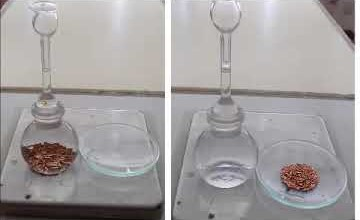
\includegraphics[width=0.50\linewidth]{imágenes/picnometriaSolido.jpg}
    
        \caption{Esquema de una picnometría de sólidos}
    \end{figure}

    Lo que tratamos de determinar con  estas medidas es la diferencia de masa entre el picnómetro lleno con solo agua y con agua y perdigones. La masa total del conjunto obedecerá la siguiente relación:
    
        \begin{equation}
            m_{T}=m_{P}+m_{s}+\rho_{o} \Delta V
            \label{RelacionMasas}
        \end{equation}
    
    Donde $\Delta V$ es el volumen del agua en el picnómetro con perdigones:

        \begin{equation}
            \Delta V = V_{P}-V_{s}=V_{P}-\frac{m_{s}}{\rho_{s}}
        \end{equation}

    Sustituyendo $\Delta V$ en la Ec.\ref{RelacionMasas} y despejando el volumen del picnómetro obtenemos:

    \begin{equation}
        V = \frac{m_{T}-m_{P}-m_{s}}{\rho_{o}}+\frac{m_{s}}{\rho_{s}}
    \end{equation}

    Igualando con la Ec.\ref{VolPicnometro} obtenemos:

    \begin{equation}
        \frac{\rho_{s}}{\rho_{o}}=\frac{m_{s}}{m_{s}+m-m_{T}}
        \label{Densidad Sólido}
    \end{equation}

    
\end{itemize}



\subsection{Viscosidad}

\begin{itemize}
    \item Viscosímetro
    \item Cronómetro
    \item Líquidos a estudiar
\end{itemize}

La segunda parte de la práctica consiste en un estudio de la viscosidad de diferentes líquidos, para los que calcularemos su coeficiente de viscosidad o viscosidad dinámica $(\eta )$. Este coeficiente se define como la fuerza por unidad de área necesaria para mantener un gradiente de velocidad unidad entre dos planos paralelos de un fluido situados a una distancia unidad. La viscosidad en el CGS (Sistema Cegesimal de Unidades, basado en el centímetro, el gramo y el segundo) es el \textbf{poise} $(g(cm\: s)^{-1})$. La otra magnitud empleada es la viscosidad cinemática, que se define como el cociente entre la viscosidad dinámica y la densidad del fluido. En el CGS se mide en \textbf{stokes} $(cm^2/s)$.

\par El coeficiente de viscosidad es inversamente proporcional a la velocidad de caída del líquido por un capilar, es decir cuánto más tarda el líquido en fluir por el capilar mayor será su viscosidad dinámica. Por tanto $\eta$ es directamente proporcional al tiempo empleado por el líquido en recorrer cierta distancia a lo largo del capilar y la fórmula que relaciona las magnitudes es la siguiente:

\begin{equation}
    \eta = k \cdot  \rho \cdot t
    \label{Viscosidad 1}
\end{equation}

Donde $\rho$ es la densidad del fluido. Para medir $\eta$ el procedimiento a seguir será medir el tiempo que tarda el fluido a estudiar en desplazarse entre las dos marcas de un viscosímetro como el de la Fig.\ref{Viscosímetro}.

\begin{figure}[h!]
    \centering
    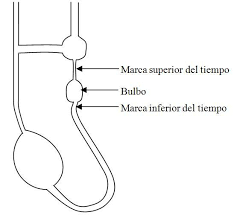
\includegraphics[width=0.4\linewidth]{imágenes/viscosimetro.png}

    \caption{Esquema de un viscosímetro}
    \label{Viscosímetro}
\end{figure}

No obstante el primer paso el conocer el valor de la constante de proporcionalidad $(k)$, independiente de cada capilar y, por tanto, independiente de cada viscosímetro. Para ello debemos trabajar con un líquido de densidad y viscosidad dinámica conocida, en nuestro caso será el agua a temperatura ambiente $T= 19,5\pm 0,5^{\circ} C$. Su coeficiente de viscosidad dinámica a la temperatura de trabajo se puede obtener a partir de la siguiente ecuación:

\begin{equation}
    \ln \frac{\eta}{\eta_{20}} = \frac{1,2348(20-T)-0,001467(T-20)^2}{T+96}
    \label{Coeficientes viscosidad}
\end{equation}

Donde $\eta_{20}$ es la viscosidad dinámica del agua a $20^{\circ}C$, que se toma como constante y tiene un valor de $0,01\: poise$.

\par Una vez conocido el valor de la viscosidad dinámica del agua a la temperatura de trabajo realizaremos diez medidas del tiempo que tarda el agua en fluir desde la marca superior hasta la marca inferior del viscosímetro. Cabe destacar que antes de realizar estas medidas se debe limpiar el viscosímetro por dentro minuciosamente, pues cualquier mota de polvo podría alterar considerablemente los tiempos medidos o incluso bloquear el agua y impedir que fluya por los capilares de forma normal.

\par Estas medidas nos servirán para determinar con mayor exactitud la constante del viscosímetro a partir de la Ec.\ref{Viscosidad 1} de la siguiente forma:

\begin{equation}
    k = \frac{\eta}{\rho \cdot t}
    \label{Coef Viscosimetro}
\end{equation}

Una vez determinada la constante del viscosímetro podemos proceder con rigor a determinar los diferentes coeficientes de viscosidad de los dos líquidos a estudiar: acetona y alcohol.

\par El procedimiento a seguir con los dos líquidos es idéntico, vamos a medir el tiempo que tardan en fluir desde la marca superior hasta la marca inferior del viscosímetro, como se observa en la Fig.\ref{Viscosímetro}. En el caso de la acetona realizamos diez medidas de ese mismo tiempo, mientras que para el alcohol solo pudieron ser realizadas siete medidas por falta de tiempo. El cálculo de la viscosidad dinámica de cada líquido se realizará a partir de la Ec.\ref{Viscosidad 1}, con su respectiva incertidumbre obtenida a partir de propagación de incertidumbres.


\newpage

\section{Análisis de datos}

\subsection{Densidad}

\subsubsection{Cálculo del volumen del picnómetro}

Como se explicó en la metodología, el primer paso de la práctica es calcular el volumen del picnómetro a partir de la Ec.\ref{VolPicnometro}. La masa del picnómetro vacío y seco es la siguiente:

\begin{equation}
    m_{p} = 19.12 \pm 0,01 \; g
\end{equation}

Donde la incertidumbre representa la precisión de la balanza empleada.

\par Para calcular el valor de la masa del picnómetro lleno de agua realizamos diez medidas y calculamos su media aritmética y su incertidumbre de tipo A y B con el siguiente tratamiento estadístico:

\begin{table}[h!]
    \centering
    \begin{tabular}{|c|c|}
    \hline
    Medida & $m \pm s(m)\; g$  \\ \hline
    $1$    & $45.74 \pm 0.01$ \\ \hline
    $2$    & $45.73 \pm 0.01$ \\ \hline
    $3$    & $45.76 \pm 0.01$ \\ \hline
    $4$    & $45.75 \pm 0.01$ \\ \hline
    $5$    & $45.78 \pm 0.01$ \\ \hline
    $6$    & $45.67 \pm 0.01$ \\ \hline
    $7$    & $45.66 \pm 0.01$ \\ \hline
    $8$    & $45.80 \pm 0.01$ \\ \hline
    $9$    & $45.78 \pm 0.01$ \\ \hline
    $10$   & $45.74 \pm 0.01$ \\ \hline
    \end{tabular}
    \caption{Medidas de la masa del picnómetro lleno de agua}
    \label{Pic Agua}
    \end{table}

La media aritmética de la muestra inicial (Con $n=10$) y su desviación típica se calculan de la siguiente forma:

\begin{align}
    \overline{m} &= \frac{\sum_{i}^n m_{i}}{n} = 45.740 \; g 
    \label{Media1} \\
    s_{A}(m) &= \sqrt{\frac{\sum_{i}^n (m_i-\overline{m})^2}{n-1}} = 0.043 \; g
    \label{Desviación Típica de la muestra}
\end{align}

La desviación típica de la media se calcula de la siguiente forma:

\begin{equation}
    s_{A}(\overline{m}) = \frac{s_{A}(m)}{\sqrt{n}} = 0.014 \; g
    \label{Desv_T_agua}
\end{equation}


El siguiente paso será establecer los intervalos de confianza para eliminar los valores discordantes y tener datos con más precisión. Los intervalos vendrán determinados por la siguiente relación: $\overline{m} \pm k \cdot s_{A}(\overline{m})$, donde $k \cdot s_{A}(\overline{m})$ representa la incertidumbre expandida y $k$ es el factor de cobertura de la distribución T de Student. En todos los análisis posteriores tomaremos $k=2$ para obtener una probabilidad del $95 \%$.

\begin{align}
    \begin{split}
        \overline{m} - k \cdot s_{A}(m) \leq &m_{i} \leq \overline{m} + k \cdot s_{A}(m) \\
        45,654 \leq &m_{i} \leq 45.826
    \end{split}
\end{align}

A continuación debemos calcular el valor de la incertidumbre combinada de la muestra, que se calcula con la desviación típica de la media, calculada en la Ec.\ref{Desv_T_agua} y la incertidumbre de tipo B, que tomaremos como la precisión de la balanza, por lo que tendrá un valor de $0,01$:

\begin{equation}
    s_{C}(\overline{m}) = \sqrt{[s_{A}(\overline{m})]^2+[s_{B}(m)]^2} = 0,017 \; g
    \label{Inc combinada}
\end{equation}

Después de aplicar el factor de cobertura podemos observar que todos los datos experimentales se encuentran dentro del intervalo de confianza por lo que el valor final de la media de la masa del picnómetro con agua es el siguiente:

\begin{equation}
    \overline{m} = 45,740 \pm 0,017 \; g
\end{equation}

Por tanto, el volumen del picnómetro tomaría el siguiente valor, aplicando la Ec.\ref{VolPicnometro}:

\begin{equation}
    V = \frac{\overline{m}-m_{p}}{\rho_{o}}  = 26.621\; mL
\end{equation}

Para calcular la incertidumbre del volumen del picnómetro vamos a aplicar propagación de incertidumbres:

\begin{align}
    \begin{split}
    s(V) = &\sqrt{\left (\frac{\partial V}{\partial \overline{m}}\right )^2 s^2(\overline{m})  + \left (\frac{\partial V}{\partial m_{p}}\right )^2 s^2(m_{p})} \\
    s(V) = &\sqrt{\left (\frac{1}{\rho_{o}}\right )^2 s^2(\overline{m})  + \left (\frac{-1}{\rho_{o}}\right )^2 s^2(m_{p})} = 0.014 \; mL
    \end{split}
\end{align}

Por tanto, el valor final del volumen del picnómetro es el siguiente:

\begin{equation}
    V = 26,621 \pm 0,014 \; mL
\end{equation}

\subsubsection{Densidad de la acetona}

Una vez conocido el volumen del picnómetro podemos proceder a determinar las densidades de diferentes sustancias, en primer lugar la acetona. Como se explicó en la metodología, el primer paso será tomar diez medidas de la masa del picnómetro lleno de acetona:

\begin{table}[h!]
    \centering
    \begin{tabular}{|c|c|}
    \hline
    Medida & $m \pm s(m) \; g$\\ \hline
    $1$    & $40.38\pm 0,01$ \\ \hline
    $2$    & $40.43\pm 0,01$ \\ \hline
    $3$    & $40.39\pm 0,01$ \\ \hline
    $4$    & $40.34\pm 0,01$ \\ \hline
    $5$    & $40.34\pm 0,01$ \\ \hline
    $6$    & $40.35\pm 0,01$ \\ \hline
    $7$    & $40.33\pm 0,01$ \\ \hline
    $8$    & $40.30\pm 0,01$ \\ \hline
    $9$    & $40.28\pm 0,01$ \\ \hline
    $10$   & $40.29\pm 0,01$ \\ \hline
    \end{tabular}
    \caption{Medidas de la masa del picnómetro lleno de acetona}
    \label{Masas Acetona}
    \end{table}

A continuación debemos realizar un tratamiento estadístico similar al que hicimos con los datos de las masas del picnómetro lleno de agua. La media y la desviación típica de la muestra se calculan con las Ec.\ref{Media1} y Ec.\ref{Desviación Típica de la muestra} respectivamente:

\begin{align}
    \overline{m}_{ac} = &40.343 \; g    \\
    s_{A}(m_{ac}) &= 0.045 \; g
\end{align}

Aplicando el factor de cobertura $k=2$ obtenemos el intervalo de confianza $[40,253 \; g ; 40,433 \; g]$, que engloba a todos nuestros datos. El siguiente paso será calcular la incertidumbre combinada (Usando la Ec.\ref{Inc combinada}) a partir de la desviación típica de la media (Usando la Ec.\ref{Desv_T_agua}) y la incertidumbre de tipo B, que tomaremos otra vez como $0,01$, el valor de la precisión de la balanza:

\begin{align}
    &s_{A}(\overline{m}_{ac}) = 0.014 \; g \\
    s_{C}(\overline{m}_{ac}) = &\sqrt{0,014^2 + 0,01^2} = 0.017 \; g
\end{align}

Por tanto, el valor final de la media de la masas del picnómetro lleno de acetona es el siguiente:

\begin{equation}
    \overline{m}_{ac} = 40,343 \pm 0,017 \; g
\end{equation}

Este valor nos servirá para calcular la densidad de la acetona a partir de la Ec.\ref{Densidad liq}:

\begin{equation}
    \frac{\rho}{\rho_o}=\frac{\overline{m}_{ac}-m_{p}}{\overline{m}-m_{p}} \Rightarrow \rho_{ac} = \frac{40,34-19,12}{45,74-19,12} = 0.79723 \; \frac{g}{cm^3}
\end{equation}

Aplicando propagación de incertidumbres podemos calcular la incertidumbre de esta medida indirecta:

\begin{gather}
    s(\rho_{ac}) = \sqrt{\left (\frac{\partial \rho_{ac}}{\partial \overline{m}_{ac}} \right )^2 s^2(\overline{m}_{ac})  +  \left (\frac{\partial \rho_{ac}}{\partial \overline{m}} \right )^2 s^2(\overline{m})  +  \left (\frac{\partial \rho_{ac}}{\partial m_{p}} \right )^2 s^2(m_{p})} \\
    s(\rho_{ac}) = \sqrt{\left (\frac{1}{\overline{m}-m_{p}} \right )^2 s^2(\overline{m}_{ac})  +  \left (\frac{-(\overline{m}_{ac}-m_{p})}{(\overline{m}-m_{p})^2} \right )^2 s^2(\overline{m})  +  \left (\frac{\overline{m}_{ac}-\overline{m}}{(\overline{m}-m_{p})^2} \right )^2 s^2(m_{p})} \nonumber  \\
    s(\rho_{ac}) = 0.00083 \; \frac{g}{cm^3} \nonumber
    \label{Inceridumbre densidad liq}
\end{gather}

Por tanto el valor final de la densidad de la acetona es:

\begin{equation}
    \rho_{ac} = 0.79723 \pm 0.00083 \; \frac{g}{cm^3}
\end{equation}

El valor real de la densidad de la acetona es de $0,784 \; \frac{g}{cm^3}$, que se encuentra bastante próximo al resultado experimental pero no entra dentro del rango de incertidumbre. Los valores de la masa del picnómetro con acetona presentan muy poca dispersión por lo que el motivo de discordancia es otro.La diferencia entre los dos valores se puede explicar probablemente por la presencia de cierta cantidad de agua en el picnómetro, sustancia de una densidad mayor que la de la acetona y que, de estar presente, aumentaría el valor experimental de la densidad. 

\newpage

\subsubsection{Densidad del alcohol}

Para determinar la densidad del alcohol procederemos igual que con la acetona. En primer lugar, las diez medidas de la masa del picnómetro lleno de alcohol son las siguientes:

\begin{table}[h!]
    \centering
    \begin{tabular}{|c|c|}
    \hline
    Medida & $m \pm s(m) \: g$   \\ \hline
    $1$    & $41.12\pm0.01$ \\ \hline
    $2$    & $41.13\pm0.01$ \\ \hline
    $3$    & $41.13\pm0.01$ \\ \hline
    $4$    & $41.12\pm0.01$ \\ \hline
    $5$    & $41.13\pm0.01$ \\ \hline
    $6$    & $41.11\pm0.01$ \\ \hline
    $7$    & $41.02\pm0.01$ \\ \hline
    $8$    & $41.07\pm0.01$ \\ \hline
    $9$    & $41.11\pm0.01$ \\ \hline
    $10$   & $41.11\pm0.01$ \\ \hline
    \end{tabular}
    \caption{Medidas de la masa del picnómetro lleno de alcohol}
    \label{Masas Alcohol}
    \end{table}

A partir de un tratamiento estadístico idéntico al que realizamos con la acetona obtuvimos el siguiente dato de incertidumbre y la media de las masas:

\begin{gather}
    \overline{m}_{al} = 41.105 \; g \\
    s_{A}(m_{al}) =  0.033 \; g 
\end{gather}

Si aplicamos el factor de cobertura $k=2$ obtenemos el intervalo de confianza $[41.039 \; g ; 41.171 \; g]$, que nos obliga a dejar fuera a la medida número 7, de $41,02 \;g$. Con estos datos podemos calcular ya la nueva media, la desviación típica de la media y la incertidumbre combinada de forma análoga a como lo hicimos con la acetona.

\begin{gather}
    \overline{m}_{al} = 41.1144 \; g\\
    s_{A}(\overline{m}_{al}) = 0.0059 \; g\\
    s_{C}(\overline{m}_{al}) = 0.012 \; g
\end{gather}

El valor final de la media de las masas del picnómetro lleno de alcohol es:

\begin{equation}
    \overline{m}_{al} = 41,114 \pm 0,012 \; g
\end{equation}

Sustituyendo este valor en la Ec.\ref{Densidad liq} podemos obtener el valor de la densidad del alcohol:

\begin{equation}
    \rho_{al}  = 0.82620 \; \frac{g}{cm^3}
\end{equation}

Por último, calcularemos la incertidumbre de la densidad del alcohol aplicando la Ec.\ref{Inceridumbre densidad liq}, sustituyendo, por supuesto, la media de las masas de la acetona por la del alcohol. De esta forma el valor final de la densidad del alcohol es:

\begin{equation}
    \rho_{al} = 0.82620 \pm 0.00069 \; \frac{g}{cm^3}
\end{equation}

El alcohol empleado en la práctica fue alcohol etílico o etanol, cuya densidad real es de $0,789 \frac{g}{cm^3}$. Este valor se encuentra también bastante próximo al experimental pero se sale del rango de incertidumbre. Esta discordancia se puede explicar de la misma forma que la anterior, la presencia de cierta cantidad agua en el picnómetro (Líquido de densidad mayor que la del alcohol) aumenta ligeramente el valor experimental de la densidad del alcohol. Como podemos observar, el ligero aumento de la densidad experimental se repite con ambos líquidos, lo que refuerza nuestras suposiciones de que la presencia de cierta cantidad de agua (Algo difícil de evitar) pueda estar causando estas variaciones.


\newpage

\subsubsection{Densidad de un sólido: El plomo}

Para determinar la densidad del plomo lo primero que hicimos fue pesar nuestros perdigones de plomo:

\begin{equation}
    m_{pe} = 9,61 \pm 0,01 \; g
\end{equation}

A continuación realizamos diez medidas de la masa del picnómetro con los perdigones lleno de agua, nuestro líquido de densidad conocida:

\begin{table}[h!]
    \centering
    \begin{tabular}{|c|c|}
    \hline
    Medida & $m \pm s(m) \; g$ \\ \hline
    $1$    & $54.42\pm0.01$ \\ \hline
    $2$    & $54.43\pm0.01$ \\ \hline
    $3$    & $54.49\pm0.01$ \\ \hline
    $4$    & $54.44\pm0.01$ \\ \hline
    $5$    & $54.49\pm0.01$ \\ \hline
    $6$    & $54.51\pm0.01$ \\ \hline
    $7$    & $54.40\pm0.01$ \\ \hline
    $8$    & $54.40\pm0.01$ \\ \hline
    $9$    & $54.46\pm0.01$ \\ \hline
    $10$   & $54.46\pm0.01$ \\ \hline
    \end{tabular}
    \caption{Medidas de la masa del picnómetro lleno de agua con los perdigones}
    \label{Masas Perdigones}
    \end{table}

El tratamiento estadístico a realizar es el mismo que en apartados anteriores:

\begin{gather}
    \overline{m}_{T} = 54.450 \; g \\
    s_{A}(m_{T}) = 0.037 \; g
\end{gather}

Aplicando el factor de cobertura $k=2$ obtenemos el intervalo $[54,376 \; g  ; 54,524 \; g]$, dentro del que se encuentran todos nuestros datos. Por tanto, podemos calcular la desviación típica de la media y la incertidumbre combinada, incluyendo la incertidumbre de tipo B, que será igual que en otros apartados $0,01$.

\begin{gather}
    s_{A}(\overline{m}_{T}) = 0.012 \; g \\
    s_{C}(\overline{m}_{T}) = 0.015 \; g
\end{gather}

\newpage

Por tanto, la media de las masas del picnómetro con perdigones y agua es la siguiente:

\begin{equation}
    \overline{m}_{T}=54,450 \pm 0,015 \; g
\end{equation}

Este valor nos servirá para calcular la densidad del plomo a partir de la Ec.\ref{Densidad Sólido}

\begin{equation}
    \frac{\rho_{s}}{\rho_{o}}=\frac{m_{s}}{m_{s}+m-m_{T}} \Rightarrow \rho_{Pb} = \frac{m_{pe}}{m_{pe}+\overline{m}-\overline{m}_{T}} = 10.6659\;  \frac{g}{cm^3}
\end{equation}

Aplicando propagación de incertidumbres podemos calcular el valor de la incertidumbre de la densidad:

\begin{gather}
    s(\rho_{Pb}) = \sqrt{\left (\frac{\partial \rho_{Pb}}{\partial m_{pe}} \right )^2 s^2(m_{pe})  +  \left (\frac{\partial \rho_{Pb}}{\partial \overline{m}} \right )^2 s^2(\overline{m})  +  \left (\frac{\partial \rho_{Pb}}{\partial \overline{m}_{T}} \right )^2 s^2(\overline{m}_{T})} \\ \textstyle
    s(\rho_{ac}) =
    \sqrt{\left (\frac{\overline{m}-\overline{m}_{T}}{(\overline{m}+m_{pe}-\overline{m}_{T})^2} \right )^2 s^2(m_{pe})  +  \left (\frac{-m_{pe}}{(\overline{m}+m_{pe}-\overline{m}_{T})^2} \right )^2 s^2(\overline{m})  +  \left (\frac{\overline{m}-\overline{m}_{T}}{(\overline{m}+m_{pe}-\overline{m}_{T})^2} \right )^2 s^2(m_{T})}\nonumber  \\
    s(\rho_{ac}) = 0.0043 \; \frac{g}{cm^3} \nonumber
\end{gather}

Por tanto el valor de la densidad del plomo es de:

\begin{equation}
    \rho_{Pb} = 10.6659 \pm 0.0043 \; \frac{g}{cm^3}
\end{equation}

El valor real de la densidad del plomo es de $11.35 \; \frac{g}{cm^3}$, que se aleja un poco del valor experimental, algo más de media unidad. La aplicación del factor de cobertura nos llevó a que trabajamos con una buena precisión, quizás el fallo se debe a la poca exactitud de los datos. Una posibilidad bastante razonable es que los perdigones no sean integramente de plomo, sino de alguna aleación que altere su densidad.

\newpage

\subsection{Viscosidad}

\subsubsection{Cálculo de la constante del viscosímetro}

A partir de la Ec.\ref{Coeficientes viscosidad} podemos determinar el valor de la viscosidad dinámica a la temperatura de trabajo despejándola de esta forma:

\begin{align}
    \begin{split}   %El split ayuda a poner solo un número
    \eta_{ag} &= \eta_{20}\: e^{\frac{1,2348(20-T)-0,001467(T-20)^2}{T+96}} \\
    \eta_{ag} &= 0.010054 \: poise
    \end{split}
\end{align}

La incertidumbre obtenida para la viscosidad dinámica del agua a la temperatura de trabajo obtenida a partir de propagación de incertidumbres es la siguiente:

\begin{align}
    \begin{split}
    s(\eta_{ag}) &= \sqrt{\left (\frac{\partial \eta_{ag}}{\partial T}\right )^2 s^2(T)} \\
    s(\eta_{ag}) &= 0,000054 \:poise
    \end{split}
\end{align}

Por tanto, el valor de la constante de viscosidad del agua a la temperatura de trabajo es el siguiente:

\begin{equation}
    0,010054 \pm 0,000054 \: poise
\end{equation}

Como se explicó en el apartado anterior, una vez conocida la viscosidad dinámica del agua a la temperatura de trabajo vamos a calcular la constante del viscosimétro. Para ello las medidas obtenidas fueron las siguientes:

\begin{table}[h!]
    \centering
    \begin{tabular}{|c|c|}
    \hline
    Medida & $T \; (s)$\\ \hline
    $1$    & $153.45$ \\ \hline
    $2$    & $156.20$ \\ \hline
    $3$    & $154.89$ \\ \hline
    $4$    & $154.54$ \\ \hline
    $5$    & $153.50$ \\ \hline
    $6$    & $154.06$ \\ \hline
    $7$    & $154.01$ \\ \hline
    $8$    & $154.27$ \\ \hline
    $9$    & $154.64$ \\ \hline
    $10$   & $154.10$ \\ \hline
    \end{tabular}
    \caption{Medidas del tiempo de flujo del agua}
    \label{Tiempos agua}
    \end{table}

    \par La incertidumbre de estos valores vendrá dada por el tiempo medio de reacción de un humano ante un estímulo visual, igual que en el apartado anterior:

    \begin{equation}
        s(T) = 0,25 \; s
    \end{equation}    

    A continuación, vamos a aplicar ciertas técnicas estadísticas para calcular la media del tiempo con su incertidumbre. En primer lugar debemos calcular la media y la desviación típica de la muestra:

    \begin{equation}
        \begin{gathered}
            \overline{T} = 154.36 \; s \\
            s_A (T) = 0.75 \; s
        \end{gathered}
    \end{equation}
    
    Ahora construiremos nuestro intervalo de confianza aplicando el factor de cobertura $k=2$. En este caso obtuvimos el intervalo $[152,86\; s;155,86\; s]$. Este intervalo deja fuera al dato $T=156,20 \; s$, por lo que deberemos calcular otra vez la media y la desviación típica de la muestra:
    
    \begin{equation}
        \begin{gathered}
            \overline{T} = 154.16 \; s \\
            s_A (T) = 0.46 \; s
        \end{gathered}
    \end{equation}
    
    A partir de estos valores calcularemos la desviación típica de la media y la incertidumbre combinada, con la que expresaremos el resultado:
    
    \begin{equation}
        \begin{gathered}
            s_A(\overline{T}) = 0.15 \; s \\
            s_C(\overline{T}) = 0.29 \; s
        \end{gathered}
    \end{equation}
    
Por tanto el valor de referencia que usaremos para el tiempo de caída fue de:
    
\begin{equation}
    T = 154.16 \pm 0.29 \; s
\end{equation}

A continuación calcularemos el valor de la constante del viscosímetro con su incertidumbre aplicando la Ec.\ref{Coef Viscosimetro}:

\begin{equation}
    k = 6.522 \cdot 10^{-5 }\pm 3.7 \cdot 10^{-7} \; \frac{poise\cdot cm^3}{g\cdot s}
\end{equation}

La incertidumbre la calculamos a partir de propagación de incertidumbres, como se detallará a continuación. Para el cálculo de esta incertidumbre supusimos una densidad del agua constante con un valor de $1 \; g\cdot cm^{-3}$:

\begin{equation}
    \begin{gathered}
        s(k) = \sqrt{\left (\frac{\partial k}{\partial \eta }\right )^2 s^2(\eta) + \left (\frac{\partial k}{\partial t}\right )^2s^2(t)} = \sqrt{\left (\frac{1}{t}\right )^2s^2(\eta) + \left (\frac{-\eta}{t^2}\right )^2s^2(t)} \\ s(k) = 3.7 \cdot 10^{-7} \; \frac{poise\cdot cm^3}{g\cdot s}
    \end{gathered}
\end{equation}

\subsubsection{Viscosidad de la acetona}

El procedimiento para determinar la viscosidad de la acetona va a ser similar al empleado en el apartado anterior, solo que ahora una vez conocida la constante del viscosímetro aplicaremos la Ec.\ref{Viscosidad 1} para calcular la viscosidad dinámica de la acetona.

\par En primer lugar necesitamos un valor de referencia para el tiempo de flujo, que obtendremos de aplicar el mismo tratamiento estadístico realizado anteriormente a los valores del tiempo de flujo medidos en el laboratorio, reflejados en la siguiente tabla:

\begin{table}[h!]
    \centering
    \begin{tabular}{|c|c|}
    \hline
    Medida   & $T \; (s)$ \\ \hline
    1  & 69,51 \\ \hline
    2  & 69,99 \\ \hline
    3  & 69,58 \\ \hline
    4  & 69,8  \\ \hline
    5  & 69,85 \\ \hline
    6  & 69,73 \\ \hline
    7  & 69,84 \\ \hline
    8  & 69,67 \\ \hline
    9  & 69,59 \\ \hline
    10 & 69,80  \\ \hline
    \end{tabular}
    \caption{Medidas del tiempo de flujo de la acetona}
    \label{T acetona}
\end{table}

La incertidumbre de estos valores vendrá dada por el tiempo medio de reacción de un humano ante un estímulo visual, igual que en el apartado anterior:

\begin{equation}
    s(T) = 0,25 \; s
\end{equation}

En primer lugar debemos calcular la media y la desviación típica de la muestra:

\begin{equation}
    \begin{gathered}
        \overline{T} = 69.74 \;s\\
        s_A(T) = 0.14 \;s
    \end{gathered}
\end{equation}

El siguiente paso es aplicar el factor de cobertura $k=2$ para obtener nuestro intervalo de confianza, en este caso $[69,46\; s;70,02\; s]$. Todos los datos medidos entran dentro del intervalo de confianza por lo que no hay que descartar ninguno. La desviación típica de la media y la incertidumbre combinada tienen los siguientes valores:

\begin{equation}
    \begin{gathered}
        s_A(\overline{T}) = 0.044 \; s \\
        s_C(\overline{T}) = 0.25 \; s
    \end{gathered}
\end{equation}

Por tanto el valor final del tiempo de flujo con su incertidumbre es:

\begin{equation}
    T_{ac} = 69.74 \pm 0.25 \; s
\end{equation}

Finalmente, aplicando la Ec.\ref{Viscosidad 1} podemos calcular la viscosidad dinámica de la acetona:

\begin{equation}
    \eta_{ac} = 0.003626 \; poise
\end{equation}

La incertidumbre de la viscosidad dinámica la calcularemos aplicando propagación de incertidumbres a la Ec.\ref{Viscosidad 1}:

\begin{equation}
    \begin{gathered}
    s\left(\eta_{ac}\right) =\sqrt{\left(\frac{\partial \eta_{ac}}{\partial k}\right)^2 s^2(k)+\left(\frac{\partial \eta_{a c}}{\partial \rho_{a c}}\right)^2 s^2\left(\rho_{ac}\right)+\left(\frac{\partial \eta_{ac}}{\partial T_{ac}}\right)^2 s^2\left(T_{a c}\right)} \\
    s\left(\eta_{a c}\right)  =\sqrt{\left(\rho_{a c} \cdot T_{a c}\right)^2 s^2(k)+\left(k \cdot T_{a c}\right)^2 s^2\left(\rho_{a c}\right)+\left(\rho_{a c} \cdot k\right)^2 s^2\left(T_{a c}\right)} \\
    s(\eta_{ac}) = 2,5 \cdot 10^{-5} \; poise
    \end{gathered}
    \label{Inc visc}
\end{equation}

Por tanto, el valor final de la viscosidad de la acetona es:

\begin{equation}
    \eta_{ac} = 0.003626 \pm 2,5 \cdot 10^{-5} \; poise
\end{equation}

El valor real de la viscosidad de la acetona a $20^{\circ} C$ es de $0,0032 \; poise$, que se acerca bastante al valor medido experimentalmente, aunque no entra dentro del intervalo de incertidumbre.

\newpage

\subsubsection{Viscosidad del alcohol}

El procedimiento con el alcohol va a ser análogo al realizado con la acetona. Los datos del tiempo de flujo medidos figurarán en la siguiente tabla:

\begin{table}[h!]
    \centering
    \begin{tabular}{|c|c|}
    \hline
    Medida  & $T \;(s)$ \\ \hline
    1 & 312,88 \\ \hline
    2 & 315,22 \\ \hline
    3 & 314,57 \\ \hline
    4 & 314,47 \\ \hline
    5 & 315,96 \\ \hline
    6 & 315,74 \\ \hline
    7 & 313,51 \\ \hline
    \end{tabular}
    \caption{Datos del tiempo de flujo del alcohol}
    \label{T alcohol}
    \end{table}

Cabe destacar que para el tiempo de flujo del alcohol solo contamos con 7 medidas, pues no pudimos realizar las diez por falta de tiempo, como mencionamos anteriormente.

\par La incertidumbre de estos valores vendrá dada por el tiempo medio de reacción de un humano ante un estímulo visual, igual que en el apartado anterior:

\begin{equation}
    s(T) = 0,25 \; s
\end{equation}    

Para determinar un valor de referencia del tiempo de flujo vamos a aplicar el mismo tratamiento estadístico que anteriormente. La media y la desviación típica de la muestra son:

\begin{equation}
    \begin{gathered}
        \overline{T} = 314.6\; s\\
        s_A(T) =  1.0 \; s
    \end{gathered}
\end{equation}

Aplicando el factor de cobertura $k=2$ obtenemos un intervalo de confianza de $[312,6 \;s;316,6\; s]$, dentro del que se encuentran todos los datos medidos. Por tanto no tenemos que descartar ningún dato y podemos proceder a calcular la desviación típica de la media y la incertidumbre combinada:

\begin{equation}
    \begin{gathered}
        s_A(\overline{T}) = 0.40 \; s \\
        s_C(\overline{T}) = 0.47 \; s
    \end{gathered}
\end{equation}

Por tanto, el valor de referencia del tiempo de flujo para el alcohol es:

\begin{equation}
    T = 314.6 \pm 0.47 \; s
\end{equation}

Aplicando las Ec.\ref{Viscosidad 1} y Ec.\ref{Inc visc} (Sustituyendo los valores relativos al alcohol) obtenemos el siguiente valor para la viscosidad dinámica del alcohol y su incertidumbre:

\begin{equation}
    \eta_{al} =  0.01695 \pm 0.00010 \; poise
\end{equation}

El valor teórico de la viscosidad del alcohol es de $0,012 \; poise$, que, aún sin entrar dentro del intervalo de incertidumbre, se acerca bastante a nuestro valor experimental.

\section{Conclusión}

Como conclusión vamos a realizar una exposición de todos los resultados obtenidos, para poder analizar los resultados de forma global. La primera parte de la práctica se centraba en el concepto de densidad de diferentes materiales, dos líquidos y un sólido. Los resultados obtenidos (Comparados con el valor real) fueron los siguientes:


\begin{table}[h!]
    \centering
    \begin{tabular}{|c|c|c|}
        \hline
        Material & $\rho  \; (g \cdot cm^{-3})$ & $\rho _E\pm s(\rho_E) \; (g \cdot cm^{-3})$ \\ \hline
        Acetona &$0, 784$ & $0,79723 \pm 0,00083$ \\ \hline
        Alcohol & $0, 789$ & $0,82620 \pm  0,00069$\\ \hline
        Plomo & $11,35$ & $10,6659 \pm 0,0043$ \\ \hline
    \end{tabular}
    \caption{Densidades reales y resultados experimentales}
\end{table}

Donde $\rho$ representa la densidad real y $\rho_E$ representa la densidad determinada experimentalmente. Como podemos observar las densidades experimentales de los líquidos se acercan considerablemente al valor real y la densidad del plomo, aunque difiere algo más, también entra dentro de un margen razonable, sobre todo considerando que los perdigones empleados probablemente no estuvieran hechos enteramente de plomo. Por tanto podemos concluír que en esta primera parte de la práctica los resultados fueron satisfactorios.

\par En la segunda parte de la práctica el objetivo fue determinar la viscosidad dinámica de los dos líquidos con los que trabajamos antes, la acetona y el alcohol. Los resultados obtenidos fueron los siguientes:

\newpage

\begin{table}[h!]
    \centering
    \begin{tabular}{|c|c|c|}
        \hline
        Material & $\eta \; (poise)$ & $\eta_E \pm s(\eta_E) \; (poise)$ \\ \hline
        Acetona & $0,0032$ & $0,003626 \pm 0,000025$ \\ \hline
        Alcohol &$0,012$ & $0,01695 \pm  0,00010$\\ \hline
    \end{tabular}
\end{table}

Los resultados obtenidos reflejan de una forma bastante fiel los valores reales de la viscosidad dinámica de ambos líquidos, a pesar de las pequeñas diferencias. Una de las posibles explicaciones para estas diferencias es el cambio de temperatura, pues la viscosidad, que es una medida de la resistencia del líquido a fluir, tiene cierta dependencia de la temperatura. Esta dependencia tiene su origen a escala molecular, cuando la temperatura aumenta, y con ello la energía térmica de las partículas, se reducen las fuerzas intermoleculares que ejercen entre sí las partículas, disminuyendo su viscosidad. En la siguiente gráfica podemos ver una representación de la viscosidad de varios líquidos, en este caso estática (Medida en $cSt$), en función de la temperatura:

\begin{figure}[h!]
    \centering
    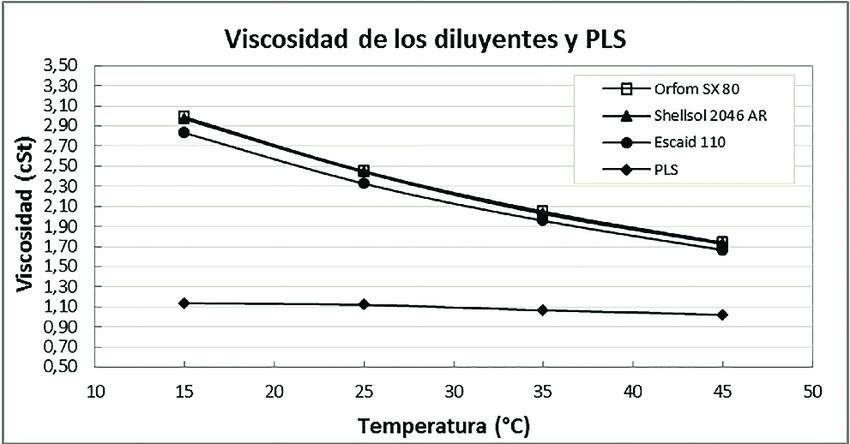
\includegraphics[width=0.65\linewidth]{imágenes/viscosidadT.png}
    \caption{Viscosidad estática de varios líquidos en función de su temperatura}
\end{figure}


Los valores de referencia de la viscosidad que aparecen en la tabla son los valores medidos a una temperatura de $20^{\circ}C$ y una presión de $ 1 \;atm$. Aunque no contamos con los datos de la temperatura de nuestro laboratorio,previsiblemente se encontraba por debajo de esos $20^{\circ}C$, por lo que es una explicación bastante razonable para que el valor de la viscosidad medido sea mayor que el real. 

\par Otra posible explicación es que el conducto del viscosímetro no estuviera suficientemente limpio, quedando alguna mota de polvo dentro de él que dificultara el flujo de los líquidos, aumentando así su viscosidad.

\par Finalmente, pese a estas pequeñas discordancias en general los resultados de las medidas se correspondían bastante con la realidad, por lo que podemos afirmar que hemos alcanzado los objetivos de la práctica. Además de eso, hemos adquirido experiencia en el manejo de aparatos como el picnómetro o el viscosímetro.


\end{document}